\documentclass{article}
\usepackage{graphicx}

\begin{document}
\bibliographystyle{plain}

\title{Spectroscopy of Magnetic B Emission Stars}

%% Use \author, \affil, and the \and command to format
%% author and affiliation information.
%% Note that \email has replaced the old \authoremail command
%% from AASTeX v4.0. You can use \email to mark an email address
%% anywhere in the paper, not just in the front matter.
%% As in the title, use \\ to force line breaks.

\author{S. Drew Chojnowski}

\vspace{0.5cm}

\section{Background}

Wisniewski et al.~\cite{wis15} presented results from optical spectroscopy of two $\sigma$ Ori E type stars discovered during the SDSS-III/APOGEE survey. $\sigma$ Ori E stars are a rare group of B stars with strong, variable magnetic fields, and weak, broad emission in the hydrogen lines. The emission is explained via the Rigidly Rotating Magnetosphere model, whereby the stellar winds are trapped a few stellar radii away at the intersections of the magnetic and rotational equators. The emission lines arise from these gaseous accumulations, which are forced to co-rotate at the rotational velocity of the stellar surface.

\begin{figure}[h!]
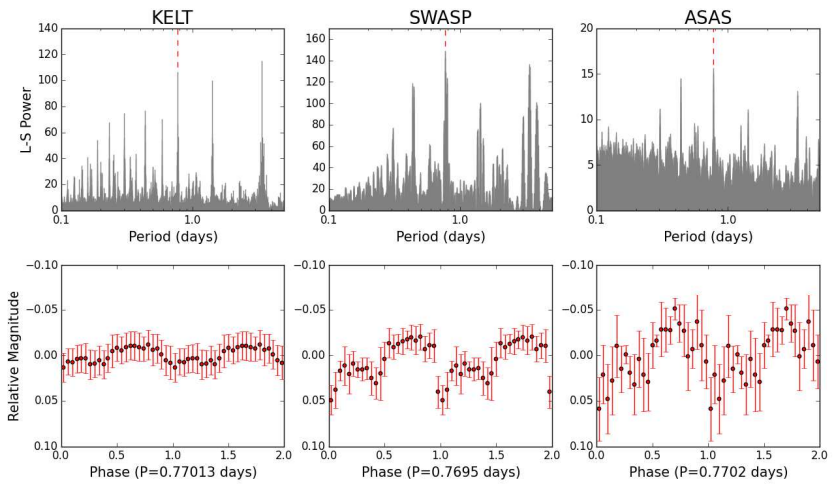
\includegraphics[angle=0,scale=.4]{Screenshot-23.png}
\caption{Phase-fold lightcurves for HD~345439. \label{fig1}}
\end{figure}

Perhaps the key result of this paper is the tentative establishment of a photometric period for the variability associated with HD~345439. Figure~\ref{fig1} shows optical lightcurves for HD~345439, folded by the estimated period of $\sim$0.77 days.



\bibliography{mybib}{}


\end{document}
